\pdfminorversion=4
\documentclass[20pt]{beamer}

\usepackage{fontspec}
\usepackage{amsfonts}
\usepackage{tangocolors}
\usepackage{hyperref}
\usepackage{multicol}
\usepackage{color}

\setbeamersize{text margin left=0pt,text margin right=0pt}

\setmainfont[Scale=0.5]{Overlock Italic}
\setsansfont[Scale=MatchLowercase]{Overlock Italic}
\setmonofont[Scale=MatchLowercase]{Fira Mono}

\setbeamertemplate{navigation symbols}{}%remove navigation symbols


\usepackage{tikz}
\usetikzlibrary{shapes}
\usetikzlibrary{backgrounds}
\usetikzlibrary{tikzmark}
\usetikzlibrary{decorations.pathmorphing}
\usetikzlibrary{positioning}
\usetikzlibrary{matrix}

%\newcommand{\tikzmark}[1]{\tikz[overlay,remember picture] \node (#1) {};}

\tikzset{
    every picture/.style={x=1em,y=1em},
    crayon/.style={very thick, line cap=round, line join=round,
          decoration={random steps, segment length=0.5pt, amplitude=0.25pt}, decorate},
    %crayon/.style={very thick},
    invisible/.style={opacity=0,line width=0,draw,text opacity=0},
    visible on/.style={alt=#1{}{invisible}},
    alt/.code args={<#1>#2#3}{%
      \alt<#1>{\pgfkeysalso{#2}}{\pgfkeysalso{#3}} % \pgfkeysalso doesn't change the path
    },
}
\tikzstyle{every picture}+=[remember picture]

\newcommand\sk{\par\bigskip\bigskip\par}

\newcommand\→{\quad}

\catcode`_=11

% http://paletton.com/#uid=70A0L0khxSyhrSYhrSYhrSYhrSY
\definecolor{bg_a}{HTML}{FFF8DA}
\definecolor{bg_b}{HTML}{FFEDDA}
\definecolor{bg_c}{HTML}{B8CFD7}
\definecolor{bg_d}{HTML}{C6C1DE}

%darker
% \definecolor{bg_a}{HTML}{D4A16A}
% \definecolor{bg_b}{HTML}{D4BF6A}
% \definecolor{bg_c}{HTML}{457585}
% \definecolor{bg_d}{HTML}{5D5393}

\newcommand\_frame[2][]{}
\newcommand\_picframe[1][]{}
\newcommand\_picframet[2][]{}

\newcommand\listing[1]{
    #1
}

\newcommand{\srcn}[2]{
    ++(0,-1) node[right,inner sep=0,outer sep=0] (#1) {
        #2 \vphantom{jJ}
    }
}
\newcommand{\src}[1]{
    \srcn{src}{#1}
}
\newcommand{\srctt}[1]{\src{\texttt{#1}}}
\newcommand{\srcttn}[2]{\srcn{#1}{\texttt{#2}}}
\newcommand{\srcttb}[1]{
    ++(0,-1) node {
        \texttt{#1} \phantom{jJ}
    }
}
\newcommand{\srcttx}[1]{\srctt{#1} {[draw,current point is local] (src.north east) -- (src.south west)}}

\newcommand\listing_z{
    node (a_up) at +(-1,1) {}
    node (a_start) {}
    \listing{
        \src{import_module(name):}
        \srcn{sys_modules_check}{\→   \texttt{sys.modules[name]}? return it}
    %[1A]
        \src{}
        \src{}
        \src{}
    %[1B]
        \srcn{find_spec}{\→   \texttt{spec = find_spec(name, path)}}
        \srcn{load}{\→   \texttt{load(spec)}}% \textcolor{tagray}{\# sets \texttt{sys.modules[name]}}}
    %[1C]
        \src{\→   \texttt{module = sys.modules[name]}}
        \src{}
        \src{}
        \src{\→   return \texttt{module}}
    }
    node (a_dn) at +(17, -1) {}
     ++(0,11)
}

\newcommand\listing_a{
    node (a_up) at +(-1,1) {}
    \listing{
        \src{import_module(name):}
        \src{\→   \texttt{sys.modules[name]}? return it}
    %[1A]
        \srcn{submoda_start}{\→   submodules:}
        \src{\→   \→   load parent module}
        \srcn{submoda_end}{\→   \→   \texttt{sys.modules[name]}? return it}
    %[1B]
        \srcn{find_spec}{\→   \texttt{spec = find_spec(name, path)}}
        \srcn{load_spec}{\→   \texttt{load(spec)}}% \textcolor{tagray}{\# sets \texttt{sys.modules[name]}}}
    %[1C]
        \src{\→   \texttt{module = sys.modules[name]}}
        \srcn{submodb_start}{\→   submodules:}
        \srcn{submodb_end}{\→   \→   set \texttt{module} as attribute of \texttt{parent}}
        \src{\→   return \texttt{module}}
    }
    node (a_dn) at +(17, -1) {}
     ++(0,11)
}
    
\newcommand\explain_load[1]{%
    \begin{tikzpicture}[overlay,opacity=0.7,text opacity=1,x=1em,y=1em]
    \path[use as bounding box] (0,0);
    \draw[draw=orange,overlay,thick,crayon,#1]
        (load.east) -- (load.east -| a_dn) coordinate (branchpt)
        (branchpt) ..controls +(0:2em) and +(180:1em).. ++(2em,0.5em)
            node[right] {\textbullet~Put module in \texttt{sys.modules}}
        (branchpt) ..controls +(0:2em) and +(180:1em).. ++(2em,-0.5em)
            node[right] {\textbullet~Initialize the module}
        ;
    \end{tikzpicture}%
}

\newcommand{\decor}[2]{
    ;
    \begin{scope}[on background layer]
        \path[#1] #2;
    \end{scope}
    \path (0,0)
}

\newcommand\decor_a{
    \decor{fill=bg_a}{(a_up) rectangle (a_dn)}
}

\newcommand\decor_z{\decor_a}

\newcommand\listing_b{
    node (b_up) at +(-1,1) {}
    \listing{
        \src{find_spec(name, path):}
%[3A]
        \src{\→    \texttt{for finder in sys.meta_path:}}
        \src{\→    \→    call its \texttt{find_spec}(name, path)}
        \src{\→    \→    return spec if successful}
%[3B]
        \src{}
        \src{PathFinder.find_spec(name, path):}
        \src{\→    \texttt{for directory in path:}}
        \src{\→    \→    get \texttt{sys.path_hooks} entry}
        \src{\→    \→    call its \texttt{find_spec}(name)}
        \src{\→    \→    return spec if successful}
    }
    node (b_dn) at +(17,-1) {}
    node (b_dnp) at +(17,-2) {}
     ++(0,10)
}

\newcommand\listing_bw{
    node (b_up) at +(-1,1) {}
    \listing{
        \src{find_spec(name, path):}
%[3A]
        \src{\→    \texttt{for finder in sys.meta_path:}}
        \src{\→    \→    call its \texttt{find_spec}(name, path)}
        \src{\→    \→    return spec if successful}
%[3B]
        \src{}
        \src{}
        \src{}
        \src{}
        \src{}
        \src{}
    }
    node (b_dn) at +(17,-1) {}
    node (b_dnp) at +(17,-2) {}
     ++(0,10)
}

\newcommand\decor_b{
    \decor{fill=bg_b}{(b_up) rectangle (b_dn)}
}
\newcommand\decor_bp{
    \decor{fill=bg_b}{(b_up) rectangle (b_dnp)}
}

\newcommand\listing_c{
    node (c_up) at +(-1,0.5) {}
    node (c_upm) at +(-1,0) {}
    \listing{
        \src{load(spec):}
        \srcn{create_a}{\→    module = \texttt{spec.loader.create_module(spec)}}
        \src{\→    if module is None:}
        \srcn{create_b}{\→    \→    module = \texttt{types.ModuleType(spec.name)}}

        \srcn{modattr}{\→    set initial module attributes}
        \src{\→    \texttt{sys.modules[spec.name]} = module}
        \srcn{exec}{\→    \texttt{spec.loader.exec_module}(module, spec)}
    }
    node (c_dn) at +(35,-1) {}
}

\newcommand\decor_c{
    \decor{fill=bg_c}{(c_up) rectangle (c_dn)}
}
\newcommand\decor_cm{
    \decor{fill=bg_c}{(c_upm) rectangle (c_dn)}
}

\newcommand\listing_d{
    node (d_up) at +(-1,0.5) {}
    node (d_upm) at +(-1,0) {}
    \listing{
        \src{get_code(module, spec):}
        \src{\→    if \texttt{spec.cached} exists, and matches \texttt{origin} stats,}
        \src{\→    \→    return it!}
        \src{\→    load source from \texttt{origin} and compile it}
        \src{\→    write bytecode to \texttt{spec.cached}}
    }
    node (d_dn) at +(35,-1) {}
    node (d_dnp) at +(35,-2) {}
}

\newcommand\decor_d{
    \decor{fill=bg_d}{(d_up) rectangle (d_dn)}
}
\newcommand\decor_dp{
    \decor{fill=bg_d}{(d_upm) rectangle (d_dnp)}
}

\newcommand\listing_a_modnoalias{
    \listing{
        \srctt{>>> import random}
        node (modnoalias) {}
        \srctt{>>> old = random}
        \srctt{}
        \srctt{>>> import random}
        \srctt{>>> random is old}
        \srctt{True}
    }
}

\newcommand\listing_a_modalias{
    \listing{
        \srctt{>>> import random}
        \srctt{>>> old = random}
        \srctt{>>> del sys.modules['random']}
        \srctt{>>> import random}
        \srctt{>>> random is old}
        \srctt{False}
        \srctt{>>> (random.sample is}
        \srctt{... \→    old.sample)}
        \srctt{False}
    }
}

\newcommand\listing_a_impostor{
    \listing{
        \srctt{>>> sys.modules['impostor'] = 'Not a module, is it?'}
        \srctt{>>> import impostor}
        \srctt{>>> impostor[:12]}
        \srctt{'Not a module'}
    }
}

\newcommand\listing_a_paths{
    \listing{
        \srctt{>>> sys.path}
        \srctt{['',}
        \srctt{ '/usr/lib64/python34.zip',}
        \srctt{ '/usr/lib64/python3.4',}
        \srctt{ ...]}
    }
}

\newcommand\listing_a_mods{
    \listing{
        \srctt{random.py           random          <- top-level module}
        \srctt{}
        \srctt{urllib/}
        \srctt{\→    __init__.py     urllib          <- package}
        \srctt{\→                                    <- top-level module}
        \srctt{\→                                    <- parent of the below}
        \srctt{\→    parse.py        urllib.parse    <-.}
        \srctt{\→    request.py      urllib.request  <-+- submodules of urllib}
        \srctt{\→    response.py     urllib.response <-'}
    }
}

\newcommand\listing_a_findspec{
    \listing{
        \srctt{if importlib.util.find_spec('foo'):}
        \srctt{\→    import foo}
        \srctt{else:}
        \srctt{\→    import fallback}
    }
}

\newcommand\listing_a_thespec{
    \listing{
        \srctt{>>> importlib.util.find_spec('antigravity')}
        \srctt{ModuleSpec(name='antigravity',}
        \srctt{\→           loader=<_frozen_importlib.SourceFileLoader ...>,}
        \srctt{\→           origin='/usr/lib64/python3.4/antigravity.py')}
    }
}

\newcommand\listing_a_record{
    \listing{
        \srctt{>>> import io}
        \srctt{>>> io.__spec__}
        \srctt{ModuleSpec(name='io',}
        \srctt{\→           loader=<_frozen_importlib.SourceFileLoader ...>,}
        \srctt{\→           origin='/usr/lib64/python3.4/io.py')}
    }
}

\newcommand\listing_a_imports{
    \listing{
        \srctt{import urllib.parse}
        \srctt{>>> urllib.__path__}
        \srctt{['/usr/lib64/python3.4/urllib']}
    }
}

\newcommand\listing_b_metapath{
    \listing{
        \srctt{>>> sys.meta_path}
        \srctt{[<BuiltinImporter>,}
        \srctt{ <FrozenImporter>,}
        \srctt{ <PathFinder>]}
    }
}

\newcommand\listing_b_pathhooks{
    \listing{
        \srctt{>>> sys.path_hooks}
        \srctt{[<zipimporter>,}
        \srctt{ <path_hook_for_FileFinder>]}
    }
}

\newcommand\listing_b_pathimportercache{
    \listing{
       \srctt{>>> sys.path_importer_cache}
       \srctt{\{'/home/petr': FileFinder('/home/petr'),}
       \srctt{ '/usr/lib64/python34.zip': <zipimporter('.../python34.zip')>,}
       \srctt{ '/usr/lib64/python3.4': FileFinder('/usr/lib64/python3.4'),}
       \srctt{ ...\}}
    }
}

\newcommand\listing_b_path{
    \listing{
        \srctt{>>> sys.path}
        \srctt{['', '/usr/lib64/python34.zip', '/usr/lib/python3.4', ...]}
    }
}

\newcommand\listing_b_exts{
    \listing{
        coordinate (col) at (+12,0)
        \srctt{random.cpython-34m.so} node[right] at (src -| col) {(Extension module)}
        \srctt{random.abi3.so} node[right] at (src -| col) {(Extension module)}
        \srctt{random.so} node[right] at (src -| col) {(Extension module)}
        \srctt{random.py} node[right] at (src -| col) {(Source module)}
        \srctt{random.pyc} node[right] at (src -| col) {(Sourceless module)}
    }
}

\newcommand\listing_b_modulespec{
    \listing{
        \srctt{ModuleSpec:}
        \srctt{\→    name}
        \src{\→\→random}
        \srctt{\→    origin}
        \src{\→\→/usr/lib64/python3.4/random.py}
        \srctt{\→    cached}
        \src{\→\→/usr/lib64/python3.4/__pycache__/random.cpython-34.pyc}
        \srctt{\→    loader}
        \src{\→\→importlib.machinery.SourceFileLoader}
        \srctt{\→    loader_state, parent, submodule_search_locations}
    }
}

\newcommand\listing_c_attrs{
    \listing{
        coordinate (col) at (+8,0)
        \srctt{spec} node[right] at (src -| col) {{\tiny$\rightarrow$} __spec__}
        \srctt{spec.name} node[right] at (src -| col) {{\tiny$\rightarrow$} __name__}
        \srctt{spec.loader} node[right] at (src -| col) {{\tiny$\rightarrow$} __loader__}
        \srctt{spec.parent} node[right] at (src -| col) {{\tiny$\rightarrow$} __package__}
        \srctt{spec.origin} node[right] at (src -| col) {{\tiny$\rightarrow$} __file__}
        \srctt{spec.cached} node[right] at (src -| col) {{\tiny$\rightarrow$} __cached__}
        \srctt{spec.submodule_search_locations}
        \srctt{} node[right] at (src -| col) {{\tiny$\rightarrow$} __path__}
     }
}

\newcommand\frame_base[1]{
    \begin{frame}
    #1
    \end{frame}
}

\newcommand\pic_base[1]{
    \begin{tikzpicture}[x=1em,y=1em]
    #1
    \end{tikzpicture}
}

\newcommand\picframe_base[1]{
    \frame_base{
        \pic_base{
        #1;
        }
    }
}

\newcommand\picframec[1]{
    \picframe_base{
        \path #1;
    }
}

\newcommand\picframet[2]{
    \frame_base{
        \pic_base{
            \path[use as bounding box] (0, 0) -- (34, -25.5);
            \path[draw=orange] #1;
        }%
        #2%
    }%
}

\newcommand\picframe[1]{
    \picframet{#1}{}
}

\begin{document}

\begin{center}
\title{Import Deep Dive}
\author{Petr Viktorin}
\date{\today}

\frame{\color{ta3gray}\LARGE
    \sk
    \textcolor{ta2gray}{Import}
    \textcolor{taskyblue}{Deep Dive}
    \sk
    \textcolor{ta2gray}{Petr Viktorin}\\[-1cm]
    \textcolor{ta2gray}{\large @\textcolor{taskyblue}{encukou}}\\[-1cm]
    \textcolor{ta2gray}{\large \textcolor{taskyblue}{encukou}@gmail.com}\\[-1cm]
    \textcolor{ta2gray}{\large \textcolor{taskyblue}{encukou}.cz}
    \sk
    \textcolor{ta2gray}{\large EuroPython 2015}
}


\picframec{
    \listing{
        \srctt{import random}
    }
}

\frame{
    Prior art

    \bigskip

    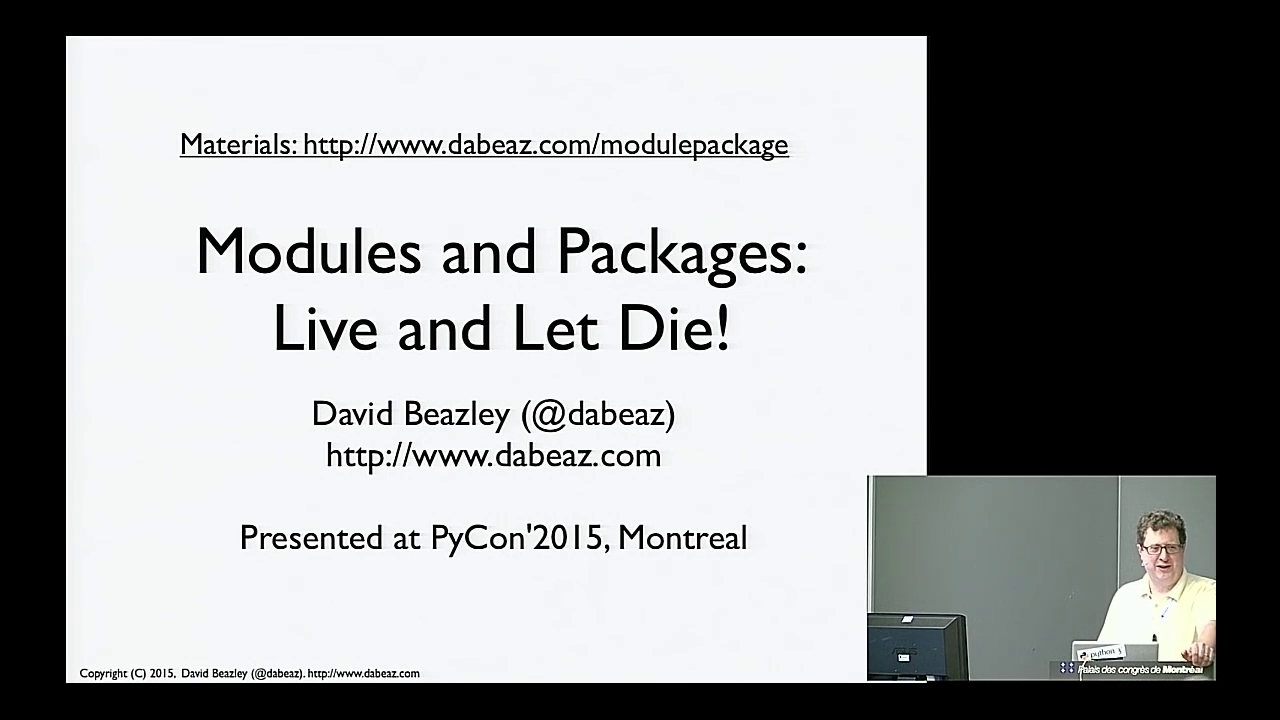
\includegraphics[width=15em]{dabeaz}

    David Beazley — Modules and Packages: Live and Let Die!\par
    \url{http://pyvideo.org/video/3387}
}

\frame[t]{
    \begin{tikzpicture}[remember picture,overlay]
    \path[use as bounding box] (0,0);
    % draw image
    \node[inner sep=0] at (current page.center)
        {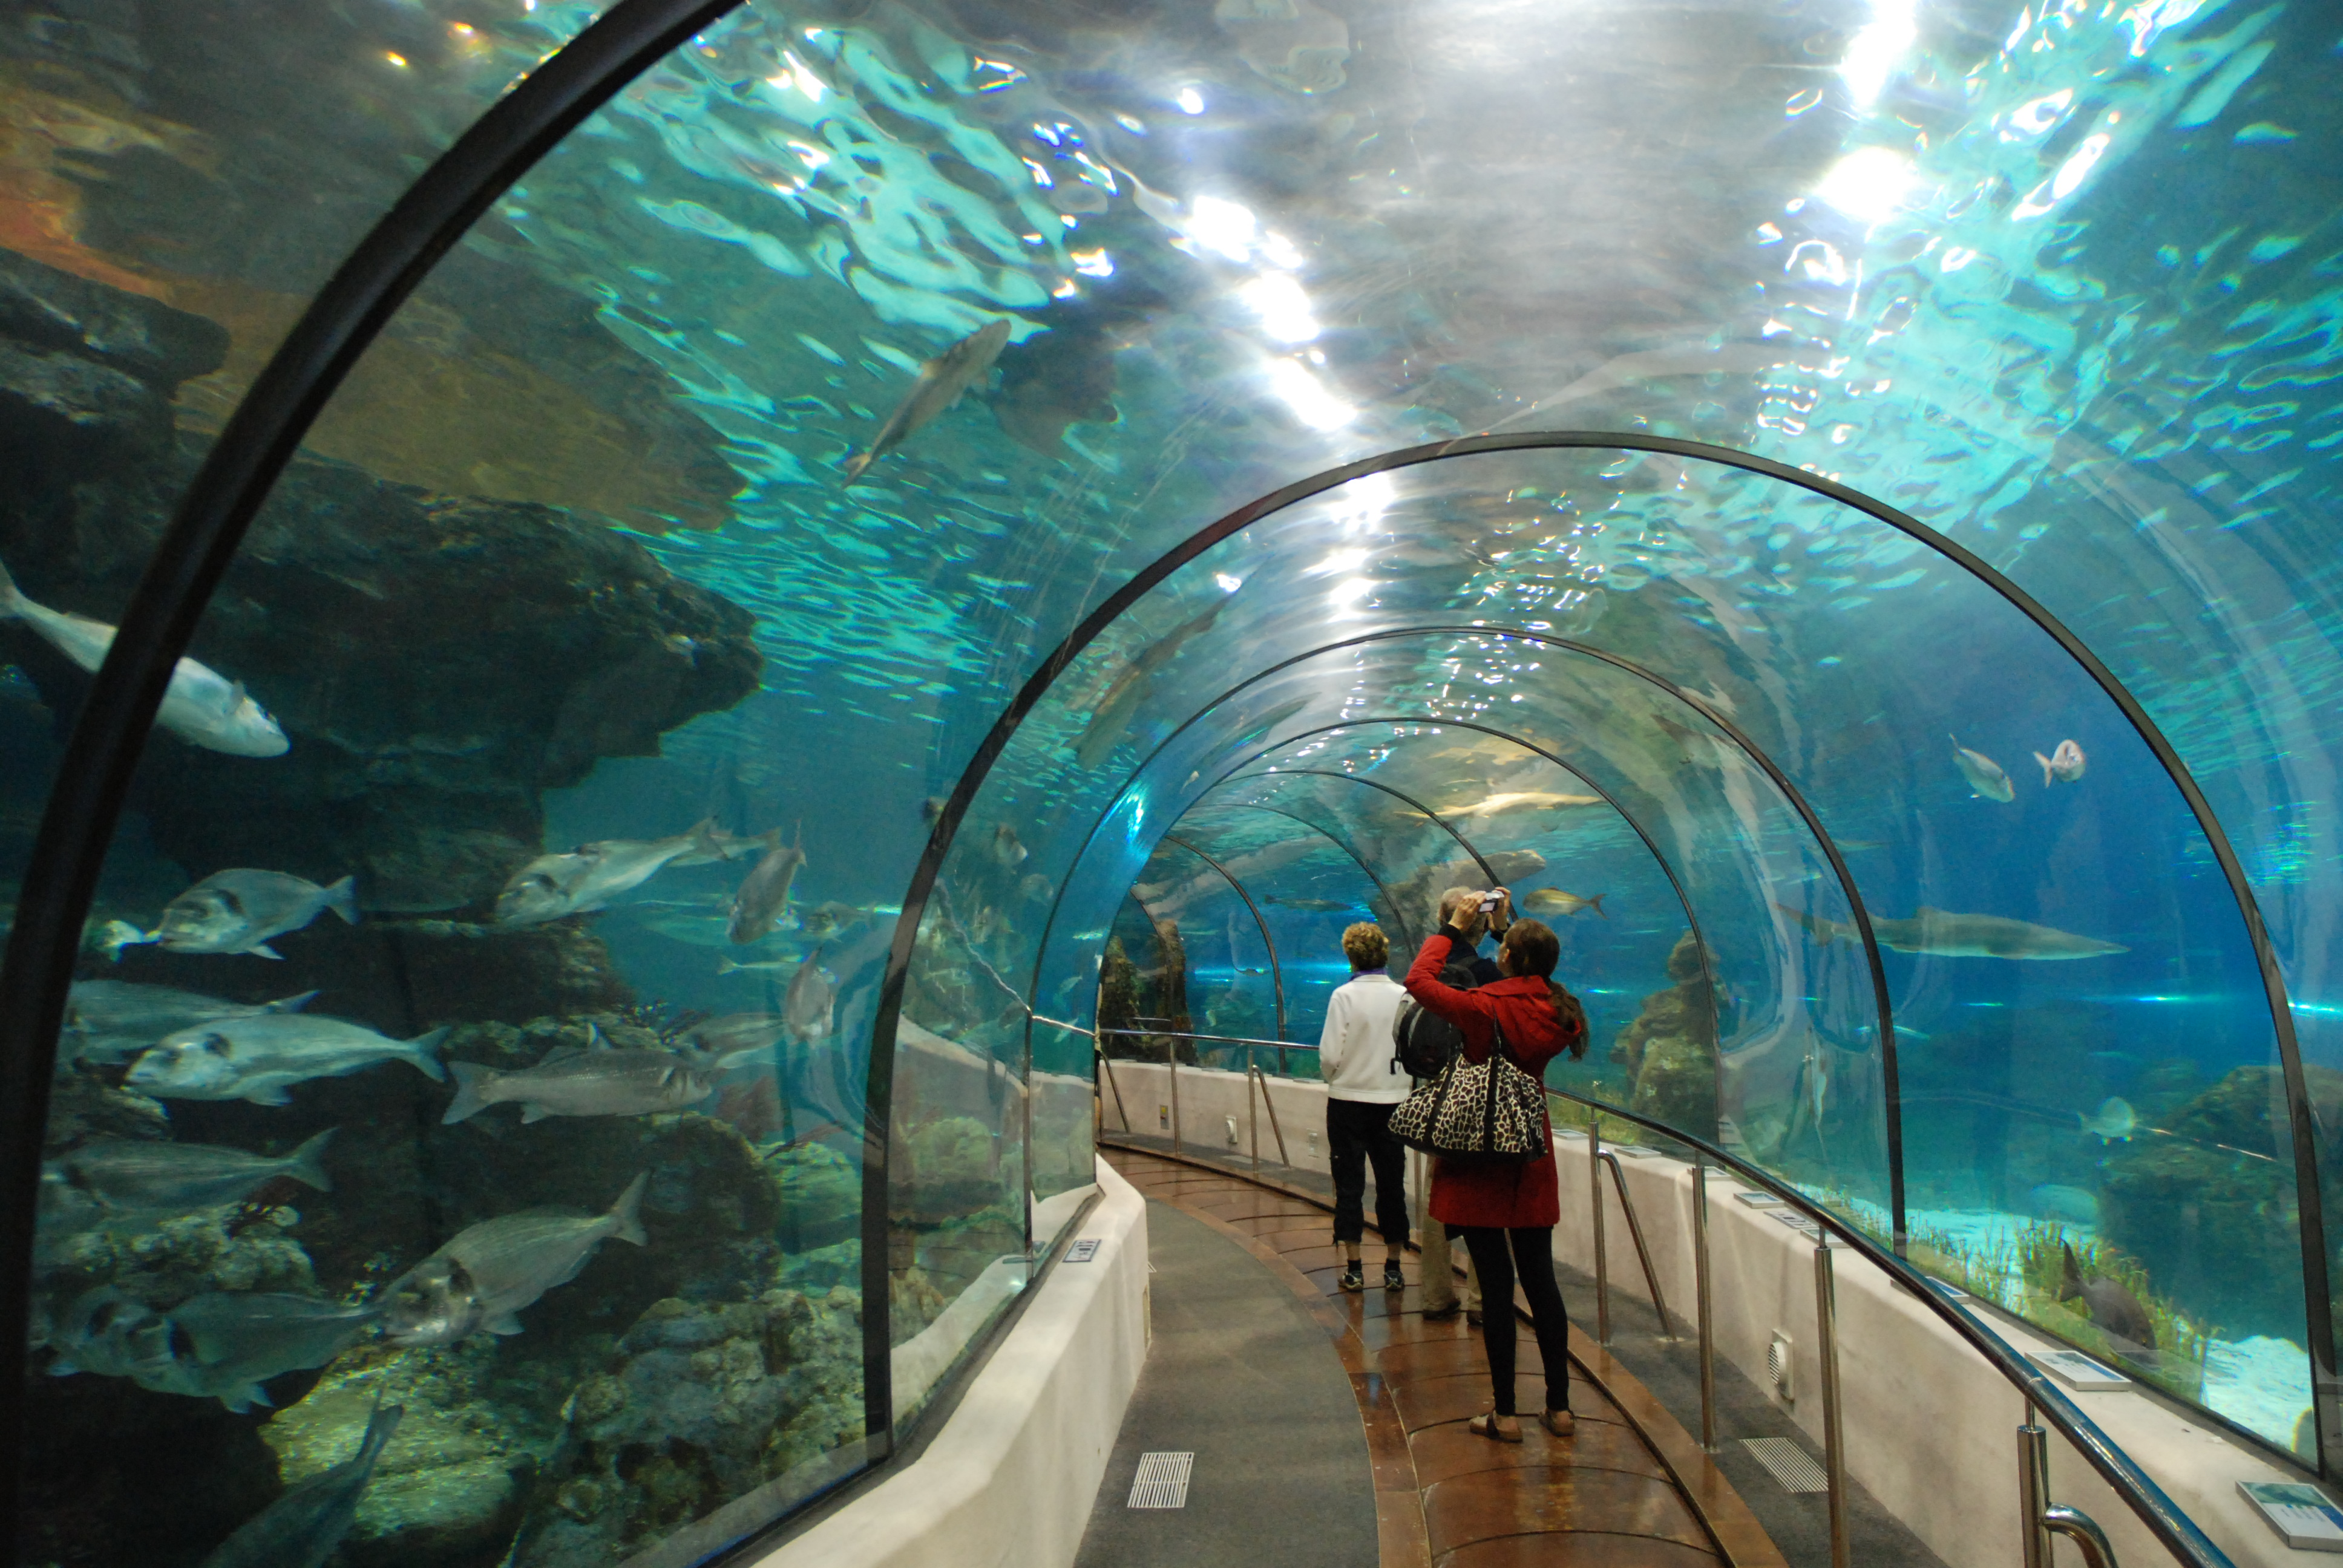
\includegraphics[width=\paperwidth,height=\paperheight]{barcelona-aquarium}};
    \node[above left,fill=black,fill opacity=0.1,text opacity=0.8]
        at(current page.south east)
        {\textcolor{white}{\tiny
               Photo © Paul Hermans, \url{https://en.wikipedia.org/wiki/File:Tunnelaquarium_14-05-2009_15-54-09.JPG}}};
    \end{tikzpicture}
}

\frame{
        \texttt{import random}

    \pause

        \texttt{random = __import__('random')}

        \bigskip
        \bigskip

    \pause
        \texttt{from
                .\tikzmark{dotdot}.sp\tikzmark{spam}am
                import
                fo\tikzmark{foo}o}

    \pause
        \bigskip

        \texttt{fo\tikzmark{fooT}o =
                __import__('sp\tikzmark{spamT}am',
                           globals(),
                           locals(),
                           ['fo\tikzmark{fooTT}o'],
                            \tikzmark{dotdotT}2).fo\tikzmark{fooTTT}o}
    \begin{tikzpicture}[remember picture,overlay]
         \path[crayon,draw,blue]
             (pic cs:fooT) +(0,1) ..controls +(90:2) and +(270:1).. (pic cs:foo) -- (pic cs:foo) ;
         \path[crayon,draw,blue]
             (pic cs:fooTT) +(0,1) ..controls +(90:2) and +(270:1).. (pic cs:foo) -- (pic cs:foo) ;
         \path[crayon,draw,blue]
             (pic cs:fooTTT) +(0,1) ..controls +(90:2) and +(270:1).. (pic cs:foo) -- (pic cs:foo) ;
         \path[crayon,draw,red]
             (pic cs:dotdotT) +(0,1) ..controls +(90:2) and +(270:1).. (pic cs:dotdot) -- (pic cs:dotdot) ;
         \path[crayon,draw,orange]
             (pic cs:spamT) +(0,1) ..controls +(90:2) and +(270:1).. (pic cs:spam) -- (pic cs:spam) ;
    \end{tikzpicture}
        \bigskip

    \small
        \url{https://docs.python.org/3/library/functions.html\#__import__}
}

\frame{
        \texttt{import \tikzmark{machi}random~}

        \texttt{random = __impo\tikzmark{machiT}rt__('random')~}

    \begin{tikzpicture}[remember picture,overlay]
         \path[<-,draw,black,semithick]
             (pic cs:machiT) +(0,1) ..controls +(90:2) and +(270:1).. (pic cs:machi) -- (pic cs:machi) ;
    \end{tikzpicture}
        \bigskip\pause
        \bigskip

        \tikz[remember picture] \node[fill=gray,fill opacity=0.25,text opacity=1] (machiTT) {The Import Machinery};

    \begin{tikzpicture}[remember picture,overlay]
         \path[<-,draw,black,semithick]
             (machiTT) ..controls +(90:2) and +(270:1).. (pic cs:machiT) -- (pic cs:machiT) ;
    \end{tikzpicture}
        \bigskip

        \bigskip\pause

        \texttt{importlib.import_\tikzmark{machiTTT}module('random')~}
    \begin{tikzpicture}[remember picture,overlay]
         \path[->,draw,black,semithick]
             (pic cs:machiTTT) +(0,1) ..controls +(90:2) and +(270:1).. (machiTT);
    \end{tikzpicture}

        \small\phantom{\texttt{jJ}}
}

\frame{
        \texttt{import \tikzmark{machi}random~}

        \texttt{~}

    \begin{tikzpicture}[remember picture,overlay]
         \path[<-,draw,black,semithick]
             (machiTT) ..controls +(90:2) and +(270:1).. (pic cs:machi) -- (pic cs:machi) ;
    \end{tikzpicture}
        \bigskip
        \bigskip

        \tikz[remember picture] \node[fill=gray,fill opacity=0.25,text opacity=1] (machiTT) {The Import Machinery};

    \begin{tikzpicture}[remember picture,overlay]
    \end{tikzpicture}
        \bigskip

        \bigskip

        \texttt{importlib.import_\tikzmark{machiTTT}module('random')~}
    \begin{tikzpicture}[remember picture,overlay]
         \path[->,draw,black,semithick]
             (pic cs:machiTTT) +(0,1) ..controls +(90:2) and +(270:1).. (machiTT);
    \end{tikzpicture}

        \small\phantom{\texttt{jJ}}
}

\frame[t]{
    \begin{tikzpicture}[remember picture,overlay]
    \path[use as bounding box] (0,0);
    % draw image
    \node[inner sep=0] at (current page.center)
        {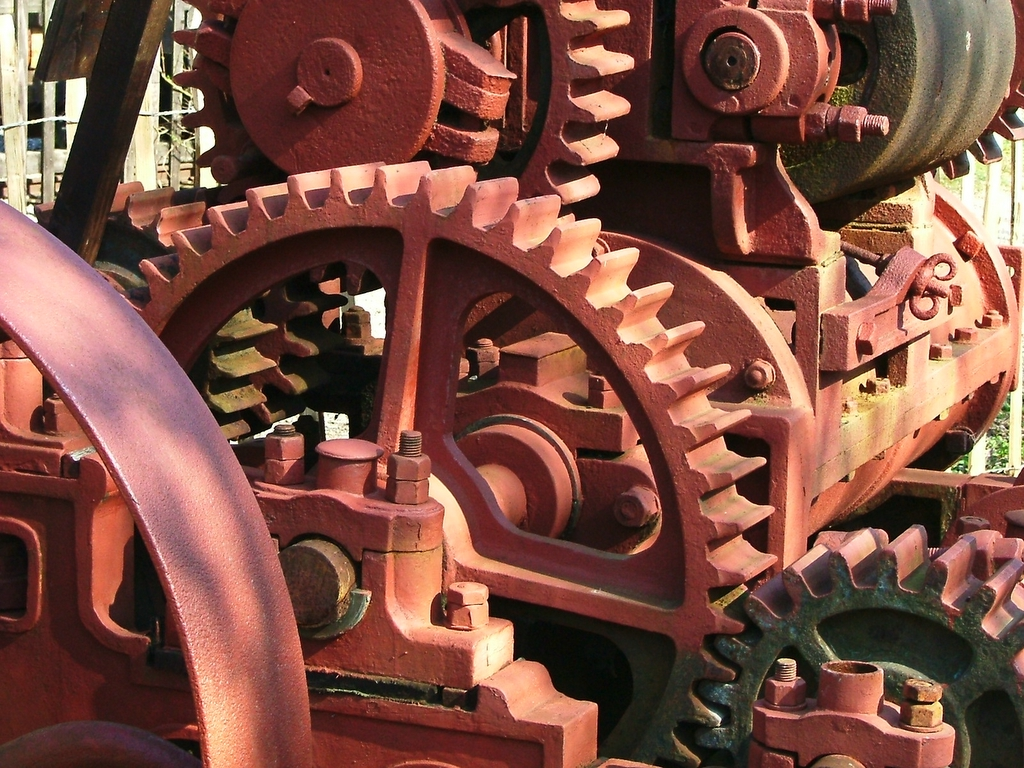
\includegraphics[width=\paperwidth,height=\paperheight]{gears}};
    \node[fill=white,fill opacity=0.75,text opacity=1] at (machiTT) {The Import Machinery};
    \node[above left,fill=black,fill opacity=0.1,text opacity=0.8]
        at(current page.south east)
        {\textcolor{white}{\tiny
               Photo © Les Chatfield, \url{https://www.flickr.com/photos/elsie/8229790}}};
    \end{tikzpicture}
    \vspace{0.5\paperheight}

    \pause

    \begin{tikzpicture}[remember picture,overlay]
        \path[fill=black,opacity=0.45]
            (machiTT.east) rectangle (20,-20)
            (machiTT.west) rectangle (-20,-20)
            (machiTT.south west) rectangle (machiTT.south east |- 0,-20);
        \node[below=1ex of machiTT] (s) {\textcolor{white}{~sans:}};
        \node[below=0pt of s] (a) {\textcolor{white}{\textbullet~Locking~}};
        \node[below=0pt of a] (b) {\textcolor{white}{\textbullet~Caching~}};
        \node[below=0pt of b] (c) {\textcolor{white}{\textbullet~Error handling~}};
        \node[below=0pt of c] (d) {\textcolor{white}{\textbullet~Pythons older than 3.4~}};
        \node[below=0pt of d] (e) {\textcolor{white}{\textbullet~Backwards compatibility shims~}};
    \end{tikzpicture}
}

\picframec{
    \listing{
        \srctt{importlib.import_module('random')}
    }
}

\picframet{
    \listing_z
    ++(18, 0)
    {[visible on=<3->]
        \listing_a_modnoalias
    }
    \decor_a
}{%
    \begin{tikzpicture}[overlay,opacity=0.7,visible on=<2->,x=1em,y=1em]
    \draw[<-,draw=orange,overlay,thick,crayon]
        (sys_modules_check.south east) rectangle (sys_modules_check.north west) ;
    \end{tikzpicture}%
}

\picframet{
    \listing_z
    ++(18, 0)
    \listing_a_modalias
    ++(-16, -5)
    {[visible on=<2->]
        \listing_a_impostor
    }
    \decor_a
}{%
    \begin{tikzpicture}[overlay,opacity=0.7,x=1em,y=1em]
    \draw[<-,draw=orange,overlay,thick,crayon]
        (sys_modules_check.south east) rectangle (sys_modules_check.north west) ;
    \end{tikzpicture}%
}
% 
% \picframe{
%     \listing_z
%     \decor_a
% }


\picframet{
    \listing_z
    ++(19, -4)
    node (path_start) at +(0,-1) {}
    {[visible on=<2->,alt=<-2>{}{text opacity=0.5}]
        \listing_a_paths
    }
    ++(-16, -5)
    {[visible on=<3->,alt=<-3>{}{text opacity=0.5}]
        \listing_a_thespec
    }
    ++(0, -1)
    {[visible on=<4->]
        \listing_a_record
    }
    \decor_a
}{%
    \begin{tikzpicture}[overlay,opacity=0.7,x=1em,y=1em]
    \path[use as bounding box] (0,0);
    \draw[<-,draw=orange,overlay,thick,crayon,visible on=<-2>]
        (find_spec.south east) ++(-1.5ex,0) node (rg) {}
        (find_spec.north east) ++(-3em,0) rectangle (rg);
    \draw[draw=orange,overlay,thick,crayon,visible on=<2>]
        (rg) ++(0,0.5em) to[bend left] (path_start);
    \draw[<-,draw=orange,overlay,thick,crayon,visible on=<3->]
        (find_spec.south west) ++(1.5ex,0) node (rg) {}
        (find_spec.north east) rectangle (rg);
    \end{tikzpicture}%
}

% \picframet{
%     \listing_z
%     ++(3, -14)
%     \listing_a_findspec
%     \decor_a
% }{%
%     \begin{tikzpicture}[overlay,opacity=0.7,x=1em,y=1em]
%     \path[use as bounding box] (0,0);
%     \draw[<-,draw=orange,overlay,thick,crayon]
%         (a_start) +(-0.5ex,0) rectangle (find_spec.south east);
%     \end{tikzpicture}%
% }

\picframet{
    \listing_z
    ++(3, -14)
    \decor_a
}{%
    \explain_load{}%
}

% \picframet{
%     \listing_z
%     ++(3, -14)
%     \decor_a
% }{%
%     \explain_load{draw=gray,draw opacity=0.5,text opacity=0.5}%
% }

\newcommand\foobar{
    \listing_z
    ++(0, -13)
    \listing{
        \src{foo.py:}
        \srctt{}
        \srcttn{imp_bar}{\→    import bar}
        \srctt{}
        \srctt{\→    bar.do_bar()}
        \srctt{}
        \srctt{\→    def do_foo():}
        \srctt{\→    \→    print('Fooing!')}
    }
    ++(18, 8)
    \listing{
        \srcn{bar}{bar.py:}
        \srctt{}
        \srcttn{imp_foo}{\→    import foo}
        \srctt{}
        \srcttn{do_foo}{\→    foo.do_foo()}
        \srctt{}
        \srctt{\→    def do_bar():}
        \srctt{\→  \→      print('Barring!')}
    }
    \decor_z
}

\picframet{
    \foobar
}{%
    \explain_load{}%
    \begin{tikzpicture}[x=1em,y=1em,draw=blue,crayon,overlay]
        \draw[->,visible on=<2->] ([yshift=3em] imp_bar.north) to (imp_bar.north);
        \draw[->,visible on=<3->] (imp_bar.north east) to (bar.west);
        \draw[->,visible on=<3->] (bar.south) to ([xshift=2em] imp_foo.north west);
        \draw[->,visible on=<4->] ([xshift=2em] imp_foo.south west) to ([xshift=2em] do_foo.north west);
        \draw[visible on=<5->,red]
            ([xshift=1ex,yshift=1ex] do_foo.east) to
            ([xshift=3ex,yshift=-1ex] do_foo.east)
            ([xshift=1ex,yshift=-1ex] do_foo.east) to
            ([xshift=3ex,yshift=1ex] do_foo.east)
            ;
    \end{tikzpicture}%
}


\picframe{
    \listing_z
    ++(3, -14)
   % \src{\huge Packages}
    \decor_a
}

\newcommand\nd[3]{
    \src{#1} node[right] (#2) at (src -| colT) {\texttt{#2}}
}
\newcommand\mod_table[1]{%
    \begin{tikzpicture}[overlay,opacity=0.7,x=1em,y=1em,text opacity=1,#1]
        \path[draw]
        coordinate (colT) at ([xshift=10em]mods_here)
        coordinate (colU) at ([xshift=23em]mods_here)
        (mods_here)
        \listing{
            \src{Filename} node[right] at (src -| colT) {Module name}
            ++(0,-0.5em)
            \nd{random.py}{random}{top-level module}
            \srctt{}
            \src{urllib/}
            \nd{\→ __init__.py}{urllib}{package}
            \nd{\→ parse.py}{urllib.parse}{submodule}
            \nd{\→ request.py}{urllib.request}{submodule}
            \nd{\→ response.py}{urllib.response}{submodule}
        }
        ;
    \end{tikzpicture}%
}
\newcommand\mod_explain[1]{%
    \begin{tikzpicture}[#1]
        \draw[draw=orange,overlay,thick,crayon]
            coordinate (d) at (random.east -| colU)
            (random.east) ..controls +(0:1)and+(180:1).. ([yshift=1em]d) node[right] (tlm) {Top-level module}
            (urllib.east) ..controls +(0:1)and+(180:1).. (tlm.west)
            ;
        \draw[draw=green,overlay,thick,crayon]
            (urllib.east) ..controls +(0:1)and+(180:1).. ([yshift=1.5em]{urllib.east -| colU}) node[right] (pkg) {Package}
            ;
        \draw[draw=green,overlay,thick,crayon]
            (urllib.east) ..controls +(0:1)and+(180:1).. ([yshift=0.25em]{urllib.east -| colU}) node[right] (par) {Parent of the below}
            ;
        \draw[draw=blue,overlay,thick,crayon]
            ({urllib.parse}.east) ..controls +(0:1)and+(180:1).. ([yshift=-1.5em]urllib.east -| colU) node[right] (sub) {Submodule}
            ({urllib.request}.east) ..controls +(0:1)and+(180:1).. (sub.west)
            ({urllib.response}.east) ..controls +(0:1)and+(180:1).. (sub.west)
            ;
    \end{tikzpicture}%
}

\picframet{
    \listing_z
    ++(2, -14)
    coordinate (mods_here)
    \decor_a
}{%
    \mod_table{opacity=1}%
    \mod_explain{overlay,opacity=0.7,x=1em,y=1em,text opacity=1}%
    \begin{tikzpicture}[overlay,x=1em,y=1em,visible on=<2->]
    \draw[<-,draw=orange,overlay,thick,crayon]
        (find_spec.south east) ++(-1.5ex,0) node (rg) {}
        (find_spec.north east) ++(-3em,0) rectangle (rg);
    \end{tikzpicture}%
}

\picframet{
    \listing_z
    ++(17.5, -3)
    \listing_a_imports
    \decor_a
}{%
    \mod_table{text opacity=0.5}%
    \mod_explain{overlay,opacity=0.2,x=1em,y=1em,text opacity=0.5}%
    \begin{tikzpicture}[overlay,x=1em,y=1em]
    \draw[<-,draw=orange,overlay,thick,crayon]
        (find_spec.south east) ++(-1.5ex,0) node (rg) {}
        (find_spec.north east) ++(-3em,0) rectangle (rg);
    \end{tikzpicture}%
}

\picframet{
    \listing_a
    ++(17.5, -3)
    \listing_a_imports
    \decor_a
}{%
    %\explain_load{draw=gray,draw opacity=0.25,text opacity=0.25}%
    \mod_table{text opacity=0.5}%
    \mod_explain{overlay,opacity=0.2,x=1em,y=1em,text opacity=0.5}%
    \begin{tikzpicture}[overlay,x=1em,y=1em]
    \draw[<-,draw=gray,opacity=0.5,overlay,thick,crayon]
        (find_spec.south east) ++(-1.5ex,0) node (rg) {}
        (find_spec.north east) ++(-3em,0) rectangle (rg);
    \end{tikzpicture}%
    \begin{tikzpicture}[overlay,x=1em,y=1em]
    \draw[draw=orange,overlay,thick,crayon]
        (submoda_start.north west) rectangle (submoda_end.south -| submodb_end.east)
        (submodb_start.north west) rectangle (submodb_end.south east)
        ;
    \end{tikzpicture}%
}

\picframet{
    \listing_a
    \decor_a
}{%
    \explain_load{}%
}

%%%%%%%%%%%%%%%%%%%%%%%%%%%%%%%%%%%%%%%%%%%%%%%%%%%%%%%%%%%%%%%%%%%%%%%%%%%%%%%

\picframet{
    \listing_a
    ++(0, -8.5)
    ++(0, -5)
    \listing{
        \srcn{init}{foo/__init__.py:}
        \src{}
        \srcttn{imp_main}{\→    from foo import main}
        \src{}
        \srcttn{imp_consts}{\→    from foo import consts}
    }
    ++(18, 5)
    \listing{
        \srcn{main}{foo/main.py:}
        \src{}
        \srcttn{imp_foo}{\→    import foo}
        \src{}
        \srcttn{use_val}{\→    use(foo.consts.value)}
    }
    ++(-18, -2)
    \listing{
        \src{foo/consts.py:}
        \srctt{\→    value = 42}
    }
    \decor_a
}{%
    \explain_load{}%
    \begin{tikzpicture}[x=1em,y=1em,draw=blue,crayon,overlay]
        \draw[->,visible on=<2->] ([yshift=1.5em] init.north) to (init.north);
        \draw[->,visible on=<3->] ([xshift=1em] init.south) to ([xshift=1em,yshift=-1em] init.south);
        \draw[->,visible on=<4->] (imp_main.north east) to (main.west);
        \draw[->,visible on=<5->] ([xshift=2em,yshift=1em] imp_foo.north west) to ([xshift=2em] imp_foo.north west);
        \draw[->,visible on=<6->] ([xshift=2em] imp_foo.south west) to ([xshift=2em] use_val.north west);
        \draw[visible on=<7->,red]
            ([xshift=1ex,yshift=1ex] use_val.east) to
            ([xshift=3ex,yshift=-1ex] use_val.east)
            ([xshift=1ex,yshift=-1ex] use_val.east) to
            ([xshift=3ex,yshift=1ex] use_val.east)
            ;
    \end{tikzpicture}%
}

\frame{
    \begin{itemize}
    \item[] \Large \texttt{__init__} should:
        \begin{itemize}
        \item[] \large import from submodules
        \item[] \large set \texttt{__all__}
        \item[] \large nothing else
        \end{itemize}
    \item[] \Large submodules should:
        \begin{itemize}
        \item[] \large not import directly from \texttt{__init__}
        \item[] \large not have internal import cycles
        \end{itemize}
    \end{itemize}
}

%%%%%%%%%%%%%%%%%%%%%%%%%%%%%%%%%%%%%%%%%%%%%%%%%%%%%%%%%%%%%%%%%%%%%%%%%%%%%%%

\picframet{
    \listing_a
    \decor_a
}{%
    \begin{tikzpicture}[x=1em,y=1em,overlay]
        \path (find_spec.west -| a_dn) ++(0.25,0)
        node[circle,fill=bg_a,text=black,draw=white,thick,inner sep=0.25ex] {?};
    \end{tikzpicture}%
}

\picframe{
    ++(0, -2)
    node at (\textwidth/2,-2) {\huge Where's the module?}

    ++(0, -2)
    \listing{
        \srctt{>>> import random}
        {[visible on=<2->]
            \srctt{>>> random}
            \srctt{<module 'random' from '/usr/lib64/python3.4/random.py'>}
        }
        {[visible on=<3->]
            \srctt{>>> random.__file__}
            \srctt{'/usr/lib64/python3.4/random.py'}
        }
    }
    ++(0, -2)

    \listing{
        {[visible on=<4->]
            \srctt{>>> import sys}
        }
        {[visible on=<5->]
            \srctt{>>> sys}
            \srctt{<module 'sys' (built-in)>}
        }
        {[visible on=<6->]
            \srctt{>>> sys.__file__}
            \srctt{Traceback (most recent call last):}
            \srctt{\→  File "<stdin>", line 1, in <module>}
            \srctt{AttributeError: 'module' object has no attribute '__file__'}
        }
    }
    ++(0, -2)

    \listing{
        {[visible on=<7->]
            \src{/usr/bin/python3}
        }
    }
}

\frame{
    \begin{tikzpicture}[x=1em,y=1em,overlay]
        \node[inner sep=0] at (current page.center)
            {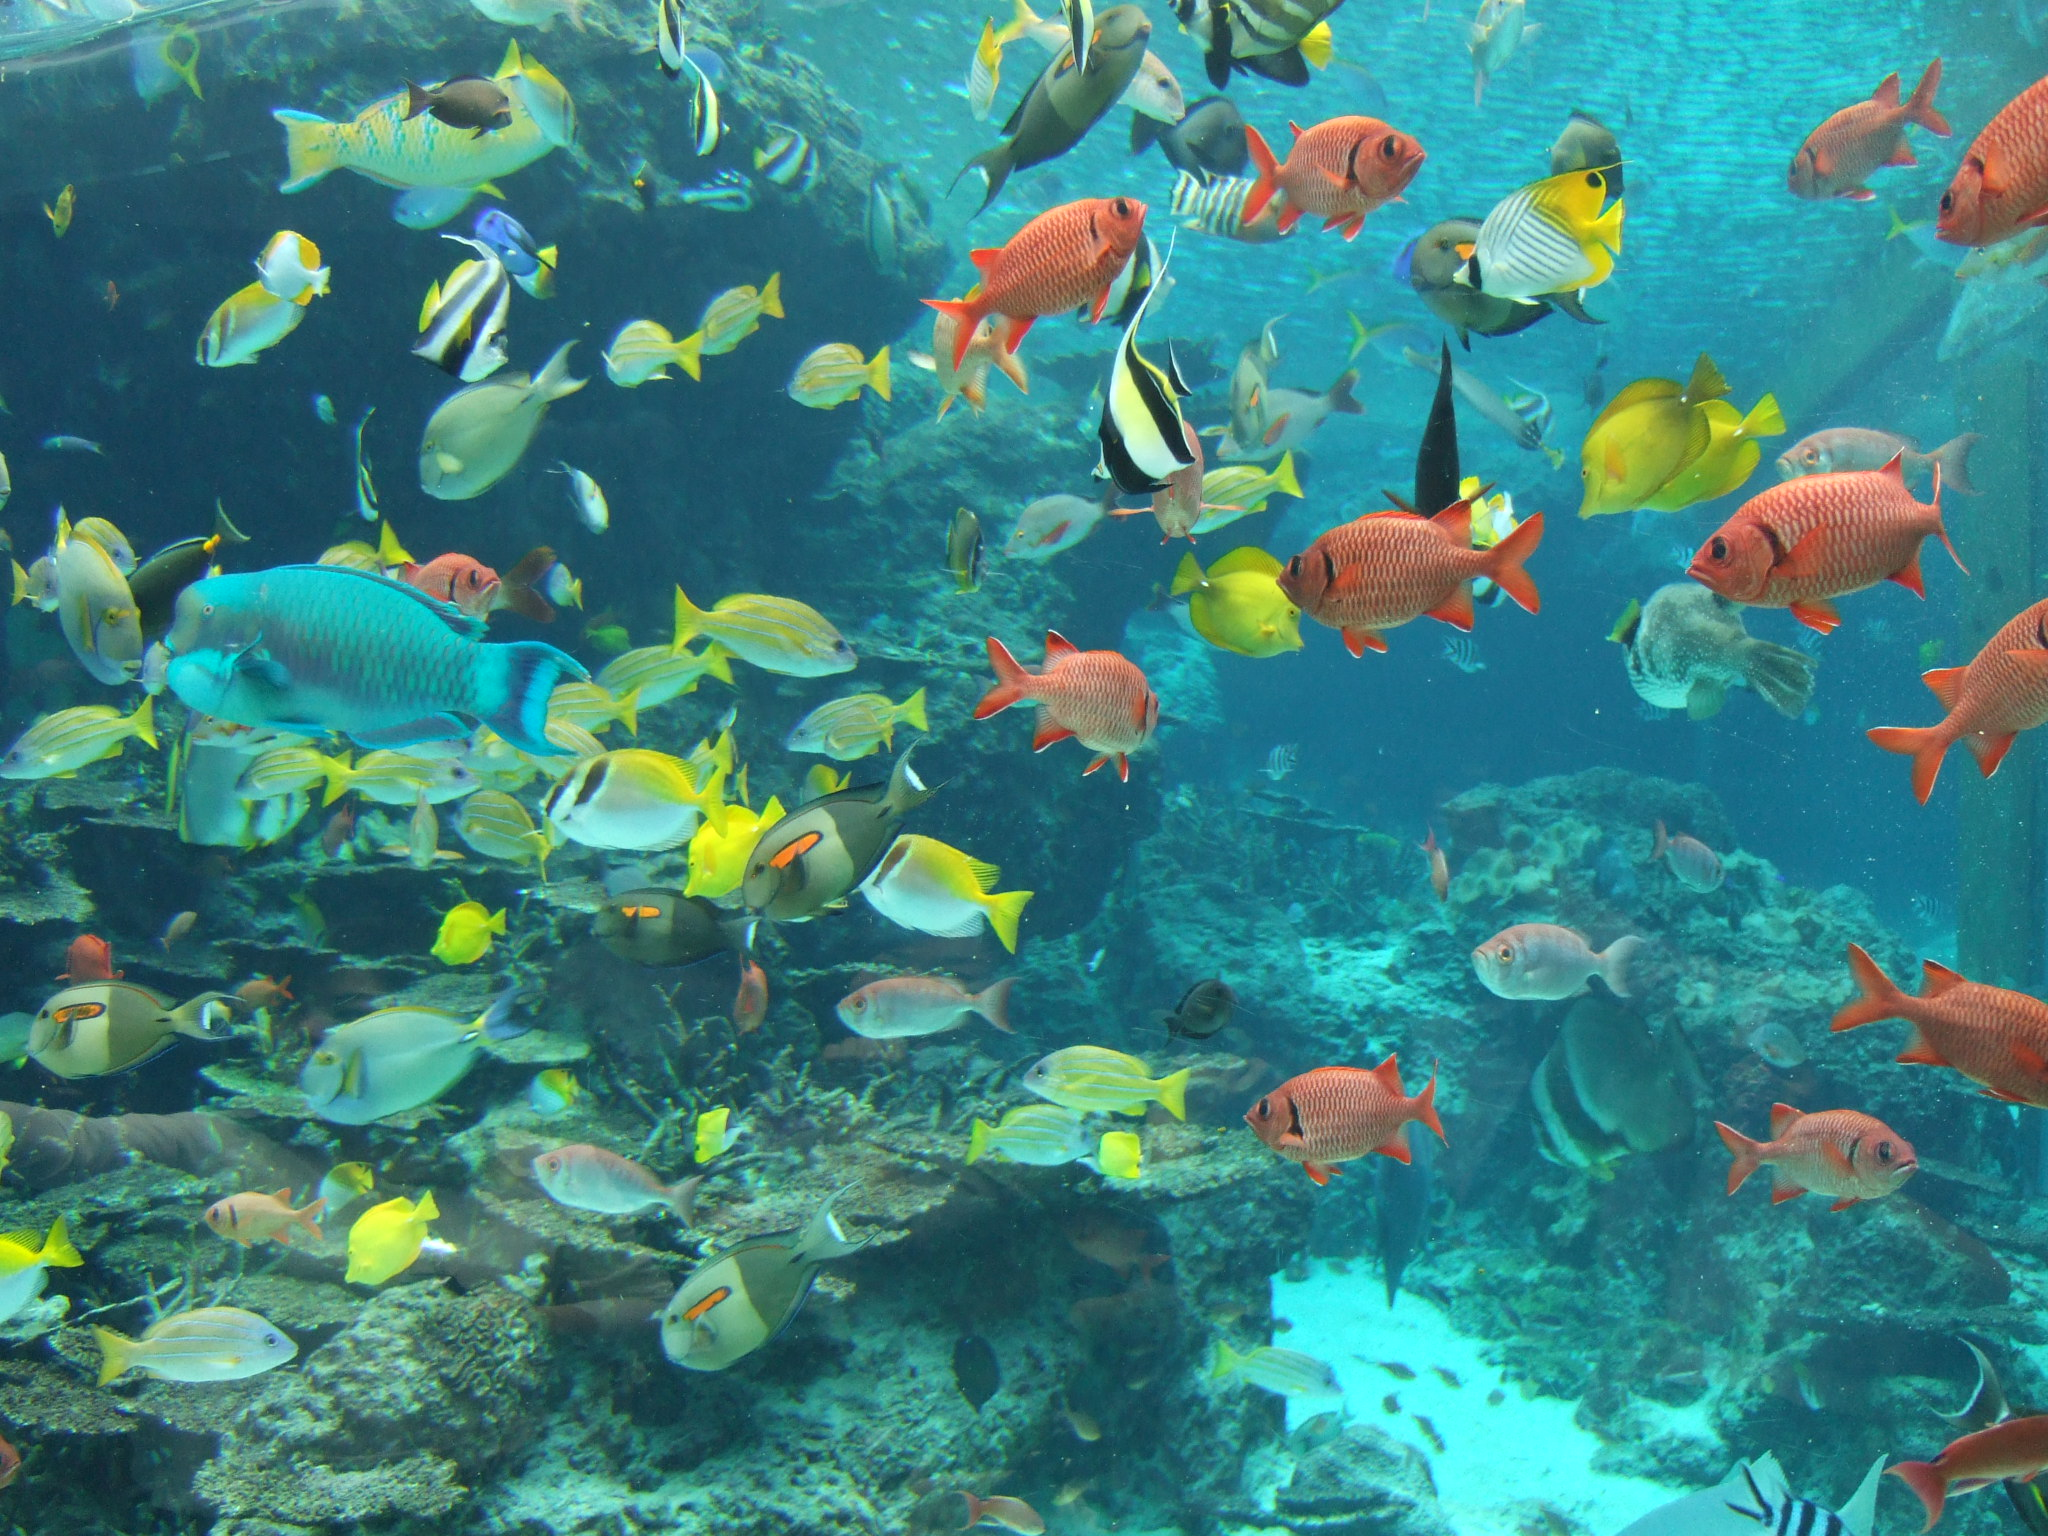
\includegraphics[width=\paperwidth,height=\paperheight]{allthefish}};
        \node[inner sep=0,minimum width=\paperwidth,minimum height=\paperheight,fill=black,opacity=0.4] at (current page.center)
            {~};
    \node[above left,fill=black,fill opacity=0.1,text opacity=0.8]
        at(current page.south east)
        {\textcolor{white}{\tiny
               Photo © Allentchang, \url{https://commons.wikimedia.org/wiki/File:Fish_in_Okinawa_Churaumi_Aquarium.JPG}}};
    \end{tikzpicture}%
    ~~~\begin{tikzpicture}[x=1em,y=1em,column sep=3mm,row sep=3mm,
                        g/.style={text=white,fill opacity=0.3,fill=black,text opacity=1,
                                  minimum width=4cm,
                                  minimum height=2cm,
                                  node font=\LARGE,
                                  },
                        gg/.style={g,minimum width=3cm},
                        f/.style={minimum width=4cm,
                                  minimum height=2cm,
                                  fill=gray!20,
                                  text=black,
                                  node font=\LARGE,
                                  }]
        \matrix (m) [ampersand replacement=\&,matrix of nodes] {
            \& |[g]| C \& |[g]| Python \\
            | [gg] | Compiled in \& | [f] | Built-in \& | [f,visible on=<3->] | Frozen \\
            | [gg] | From File \& | [f,visible on=<2->] | Extension \& | [f] | Source \\
        };
        \node[below] at ([yshift=-1ex] m-2-2.base) {\texttt{sys}};
        \node[below,visible on=<3->] at ([yshift=-1ex] m-2-3.base) {\texttt{_frozen_importlib}};
        \node[below,visible on=<2->] at ([yshift=-1ex] m-3-2.base) {\texttt{math}};
        \node[below] at ([yshift=-1ex] m-3-3.base) {\texttt{random}};
        %\path[use as bounding box] (m-2-2.south east) -- (m-3-3.north west);
    \end{tikzpicture}
}

\picframe{%
    ++(18, 0)
    \listing_b_metapath
}

\picframe{
    \listing_bw
    ++(18, 0)
    \listing_b_metapath
    \decor_b
}

\picframe{
    \listing_bw
    ++(18, 0)
    \listing_b_metapath
    ++(0, -2)
    ++(-18, -6)
    \listing_b_path
    \decor_b
}

\picframe{
    \listing_bw
    ++(18, 0)
    \listing_b_metapath
    ++(0, -2)
    \listing_b_pathhooks
    ++(-18, -3)
    \listing_b_path
    \decor_b
}

\picframe{
    \listing_b
    ++(18, 0)
    \listing_b_metapath
    ++(0, -2)
    \listing_b_pathhooks
    ++(-18, -3)
    \listing_b_path
    \decor_b
}

\picframe{
    \listing_b
    ++(18, 0)
    \listing_b_metapath
    ++(0, -2)
    \listing_b_pathhooks
    ++(-18, -3)
    \listing_b_path
    ++(0, -2)
    \listing_b_exts
    \decor_b
}

% \picframe{
%     \listing_b
%     ++(18, 0)
%     \listing_b_metapath
%     ++(0, -2)
%     \listing_b_pathhooks
%     ++(-18, -3)
%     \listing_b_pathimportercache  % can go?
%     \decor_b
% }

\picframe{
    \listing_b
    ++(0, -12)
    \listing_b_modulespec
    \decor_b
}

\picframet{
    \listing_a
    \decor_a
}{%
    \begin{tikzpicture}[x=1em,y=1em,overlay]
        \path (load_spec.west -| a_dn) ++(0.25,0)
        node[circle,fill=bg_a,text=black,draw=white,thick,inner sep=0.25ex] {?};
    \end{tikzpicture}%
}

\picframet{
    \listing_c
    \decor_c
}{%
    \begin{tikzpicture}[overlay,opacity=0.7,visible on=<2->,x=1em,y=1em]
    \draw[<-,draw=orange,overlay,thick,crayon]
        (create_a.north east) rectangle (create_b.south west) ;
    \end{tikzpicture}%
}

\picframet{
    \listing_c
    ++(0, -4)
    \listing_c_attrs
    \decor_c
}{%
    \begin{tikzpicture}[overlay,opacity=0.7,x=1em,y=1em]
    \draw[<-,draw=orange,overlay,thick,crayon]
        (modattr.north east) rectangle (modattr.south west) ;
    \end{tikzpicture}%
}

\picframe{
    \listing_c
    ++(0, -4)
    {[text=gray]
        \listing_c_attrs
    }
    ++(20, 8)
    \listing{
        \srctt{>>> import __main__}
        \srctt{>>> a = 'hello'}
        \srctt{>>> __main__.a}
        \srctt{'hello'}
        \srctt{>>> __main__.a = 'world'}
        \srctt{>>> a}
        \srctt{'world'}
    }
    \decor_c
}

\picframe{
    \listing_c
    ++(0, -4)
    {[text=gray]
        \listing_c_attrs
    }
    ++(20, 8)
    \listing{
        \srctt{>>> import __main__}
        \srctt{>>> a = 'hello'}
        \srctt{>>> __main__.a}
        \srctt{'hello'}
        \srctt{>>> __main__.a = 'world'}
        \srctt{>>> a}
        \srctt{'world'}
    }
    ++(-10, -4)
    \listing{
        \srctt{if __name__ == '__main__'}
    }
    \decor_c
}

\picframet{
    \listing_c
    ++(0, -4)
    {[text=gray]
        \listing_c_attrs
        ++(20, 8)
        \listing{
            \srctt{>>> import __main__}
            \srctt{>>> a = 'hello'}
            \srctt{>>> __main__.a}
            \srctt{'hello'}
            \srctt{>>> __main__.a = 'world'}
            \srctt{>>> a}
            \srctt{'world'}
        }
        ++(-10, -4)
        \listing{
            \srctt{if __name__ == '__main__'}
        }
    }
    \decor_c
}{%
    \begin{tikzpicture}[overlay,opacity=0.7,x=1em,y=1em]
    \draw[<-,draw=orange,overlay,thick,crayon]
        (exec.north east) rectangle (exec.south west) ;
    \end{tikzpicture}%
}

% \picframet{
%     \listing_c
%     ++(0, -4)
%     {[text=gray]
%         \listing_c_attrs
%         ++(20, 8)
%         \listing{
%             \srctt{>>> import __main__}
%             \srctt{>>> a = 'hello'}
%             \srctt{>>> __main__.a}
%             \srctt{'hello'}
%             \srctt{>>> __main__.a = 'world'}
%             \srctt{>>> a}
%             \srctt{'world'}
%         }
%         ++(-10, -4)
%         \listing{
%             \srctt{if __name__ == '__main__'}
%         }
%         ++(5, 14)
%     }
%     \listing{
%         \srctt{exec(code, module.__dict__)}
%     }
%     \decor_c
% }{%
%     \begin{tikzpicture}[overlay,opacity=0.7,x=1em,y=1em]
%     \draw[<-,draw=orange,overlay,thick,crayon]
%         (exec.north east) rectangle (exec.south west) ;
%     \end{tikzpicture}%
% }

\picframe{
    \listing_c
    ++(4, -8)
    \src{{\textbullet} Put module in \texttt{sys.modules}}
    \src{{\textbullet} Initialize the module}
    \decor_c
}

\picframe{
    \listing_d
    ++(0, -2)
    \listing{
        \srctt{ModuleSpec:}
        \srctt{\→    name}
        \src{\→\→random}
        \srctt{\→    origin}
        \src{\→\→/usr/lib64/python3.4/random.py}
        \srctt{\→    cached}
        \src{\→\→/usr/lib64/python3.4/__pycache__/random.cpython-34.pyc}
        \src{\→...}
    }
    \decor_d
}

\picframe{
    \listing_d
    ++(0, -4)
    \src{\huge Python 2}\src{}
    \listing{
        \srctt{somemodule.py}
        \srctt{somemodule.pyc}
    }
    \decor_d
}

\picframe{
    \listing_d
    ++(0, -4)
    \src{\huge Python 2}\src{}
    \listing{
        \srcttx{somemodule.py}
        \srctt{somemodule.pyc}
    }
    \decor_d
}

\picframe{
    \listing_d
    ++(0, -4)
    \src{\huge Python 2}\src{}
    \listing{
        \srcttx{somemodule.py}
        \srctt{somemodule.pyc}
    }
    ++(16, 4)
    \src{\huge Python 3}\src{}
    \listing{
        \srctt{somemodule.py}
        \srctt{__pycache__/}
        \srctt{\→\→somemodule.cpython-34.pyc}
    }
    \decor_d
}

\picframe{
    \listing_d
    ++(0, -4)
    \src{\huge Python 2}\src{}
    \listing{
        \srcttx{somemodule.py}
        \srctt{somemodule.pyc}
    }
    ++(16, 4)
    \src{\huge Python 3}\src{}
    \listing{
        \srctt{somemodule.py}
        \srctt{__pycache__/}
        \srctt{\→\→somemodule.cpython-34.pyc} coordinate (q) at ([xshift=-1ex] src.south east)
        \src{}
        \src{Or:}
        \src{}
        \srcttx{somemodule.py}
        \srctt{somemodule.pyc}
        {[draw,->=stealth,bend left] (q) to[->] (src.east)}
    }
    \decor_d
}

\picframe{
    \listing_a
    ++(18, 0)
    \listing_b
    ++(-18, -12)
    \listing_c
    ++(0, -1)
    \listing_d
    \decor_a
    \decor_bp
    \decor_cm
    \decor_dp
}

\frame{
    \begin{tikzpicture}[x=1em,y=1em,column sep=3mm,row sep=3mm,
                        f/.style={minimum width=3cm,
                                  minimum height=1.5cm,
                                  fill=gray!20,
                                  }]
        \matrix (m) [ampersand replacement=\&,matrix of nodes,overlay] {
            \& C \& Python \& Bytecode \\
            | [left] | Compiled-in \& | [f] | Built-in \& \& | [f] | Frozen \\
            | [left] | From File \& | [f] | Extension \& | [minimum width=2cm] | ~ \& | [f] | Sourceless \\
            | [left] | Zip file \& \& | [f,minimum width=2cm] | zip source \& | [f] | zip sourceless \\
        };
        \path[use as bounding box] (m-2-2.south east) -- (m-3-3.north west);
        \node[f,minimum width=3cm,minimum height=1cm,draw=white,line width=1mm]
            at ([xshift=0.5cm] m-3-3.center) {Source};
    \end{tikzpicture}

}

\end{center}
\end{document}
